\documentclass[a4paper,14pt]{extarticle}

\usepackage[utf8x]{inputenc}
\usepackage[T1]{fontenc}
\usepackage[russian]{babel}
\usepackage{hyperref}
\usepackage{indentfirst}
\usepackage{here}
\usepackage{array}
\usepackage{graphicx}
\usepackage{grffile}
\usepackage{caption}
\usepackage{subcaption}
\usepackage{chngcntr}
\usepackage{amsmath}
\usepackage{amssymb}
\usepackage{pgfplots}
\usepackage{pgfplotstable}
\usepackage[left=2cm,right=2cm,top=2cm,bottom=2cm,bindingoffset=0cm]{geometry}
\usepackage{multicol}
\usepackage{multirow}
\usepackage{titlesec}
\usepackage{listings}
\usepackage{color}
\usepackage{longtable}
\usepackage{enumitem}
\usepackage{cmap}
\usepackage{tikz}

\usetikzlibrary{shapes,arrows}

\definecolor{green}{rgb}{0,0.6,0}
\definecolor{gray}{rgb}{0.5,0.5,0.5}
\definecolor{purple}{rgb}{0.58,0,0.82}

\lstset{
	language={C},
	inputpath={../},
	backgroundcolor=\color{white},
	commentstyle=\color{green},
	keywordstyle=\color{blue},
	numberstyle=\scriptsize\color{gray},
	stringstyle=\color{purple},
	basicstyle=\small,
	breakatwhitespace=false,
	breaklines=true,
	captionpos=b,
	keepspaces=true,
	numbers=left,
	numbersep=5pt,
	showspaces=false,
	showstringspaces=false,
	showtabs=false,
	tabsize=8,
	frame=single,
}

\renewcommand{\le}{\ensuremath{\leqslant}}
\renewcommand{\leq}{\ensuremath{\leqslant}}
\renewcommand{\ge}{\ensuremath{\geqslant}}
\renewcommand{\geq}{\ensuremath{\geqslant}}
\renewcommand{\epsilon}{\ensuremath{\varepsilon}}
\renewcommand{\phi}{\ensuremath{\varphi}}
\renewcommand{\thefigure}{\arabic{figure}}
\def\code#1{\texttt{#1}}

\titleformat*{\section}{\large\bfseries} 
\titleformat*{\subsection}{\normalsize\bfseries} 
\titleformat*{\subsubsection}{\normalsize\bfseries} 
\titleformat*{\paragraph}{\normalsize\bfseries} 
\titleformat*{\subparagraph}{\normalsize\bfseries} 

\counterwithin{figure}{section}
\counterwithin{equation}{section}
\counterwithin{table}{section}
\newcommand{\sign}[1][5cm]{\makebox[#1]{\hrulefill}}
\newcommand{\equipollence}{\quad\Leftrightarrow\quad}
\newcommand{\no}[1]{\overline{#1}}
\graphicspath{{figs/}}
\captionsetup{justification=centering,margin=1cm}
\def\arraystretch{1.3}
\setlength\parindent{5ex}
\titlelabel{\thetitle.\quad}

\setitemize{itemsep=0em}
\setenumerate{itemsep=0em}

\tikzstyle{startstop} = [
	rectangle,
	align=center,
	rounded corners,
	text width=10em,
	text centered,
	draw=black
]
\tikzstyle{process} = [
	rectangle,
	align=center,
	text width=20em,
	text centered,
	draw=black
]
\tikzstyle{decision} = [
	diamond,
	aspect=4,
	align=center,
	inner sep=0pt,
	text width=10em,
	text centered,
	node distance=5em,
	draw=black
]
\tikzstyle{line} = [
	draw=black,
	thick,
	->,
	>=stealth,
	-latex'
]

\begin{document}

\begin{titlepage}
\begin{center}
	САНКТ-ПЕТЕРБУРГСКИЙ ПОЛИТЕХНИЧЕСКИЙ УНИВЕРСИТЕТ\\ ПЕТРА ВЕЛИКОГО\\[0.3cm]
	\par\noindent\rule{10cm}{0.4pt}\\[0.3cm]
	Институт компьютерных наук и технологий \\[0.3cm]
	Кафедра компьютерных систем и программных технологий\\[4cm]
	
	Отчет по лабораторной работе\\[3mm]
	Дисциплина: <<Технологии компьютерных сетей>>\\[3mm]
	Тема: <<Программирование сокетов протоколов TCP и UDP>>\\[7cm]
\end{center}

\begin{flushleft}
	\hspace*{5mm} Выполнил студент гр. 43501/3  \hspace*{2.5cm}\sign[3cm]\hfill А.Ю. Ламтев\\
	\hspace*{10.4cm} (подпись)\\[3mm]
	\hspace*{5mm} Преподаватель \hspace*{6.0cm}\sign[3cm]\hfill А.В. Зозуля\\
	\hspace*{10.4cm} (подпись)\\[3mm]
	\hspace*{11.1cm} <<\sign[7mm]>> \sign[27mm] \the\year\hspace{1mm} г.
\end{flushleft}

\vfill

\begin{center}
	Санкт-Петербург\\
	\the\year
\end{center}
\end{titlepage}
\addtocounter{page}{1}

\tableofcontents
\newpage

\section{Задание}

\subsection{Формулировка}

Разработать приложение-сервер <<Удаленный калькулятор>>, позволяющее по запросу выполнять математические операции, и удаленный клиент для сервера.

\subsection{Основные возможности}

Серверное приложение должно реализовывать следующие функции:

\begin{enumerate}
	\item Прослушивание определенного порта
	\item Обработка запросов на подключение по этому порту от клиентов
	\item Поддержка одновременной работы нескольких клиентов через механизм нитей
	\item Приём <<быстрых>> операций с аргументами от клиента. Должны поддерживаться следующие операции: сложение, вычитание, умножение,
деление
	\item Вычисление <<долгих>> математических операций (факториал, квадратный корень) с последующей отложенной посылкой результата клиенту (отдельная операция, инициируемая сервером).
	\item Обработка запроса на отключение клиента
	\item Принудительное отключение клиента
\end{enumerate}

Клиентское приложение должно реализовывать следующие функции:

\begin{enumerate}
	\item Установление соединения с сервером
	\item Посылка операции с аргументами на вычисление
	\item Получение результата вычислений <<быстрых>> операций
	\item Получения результата вычислений <<долгих>> операций
	\item Разрыв соединения
	\item  Обработка ситуации отключения клиента сервером
\end{enumerate}

\subsection{Настройки приложений}

Разработанное клиентское приложение должно предоставлять пользователю настройку IP-адреса или доменного имени удалённого калькулятора и номера порта, используемого сервером. Разработанное серверное приложение должно предоставлять пользователю настройку времени выполнения <<долгих>> операций. 

\subsection{Методика тестирования}

Для тестирования приложений запускается сервер <<Удаленного калькулятора>> и несколько клиентов. В процессе тестирования проверяются основные возможности калькулятора по мгновенному и отложенному выполнению удалённых операций. 

\section{Прикладной протокол}
%Описание форматов команд и ответов (например, в табличном виде: набор и формат команд, размеры полей, сообщения об ошибках). Прикладной протокол не зависит от нижележащего транспортного протокола, а также от языка и технологии программирования.

Разработанный протокол является бинарным, формат сообщения представлен на рис. \ref{fig:calc-prot}.

\begin{figure}[H]
	\centering
	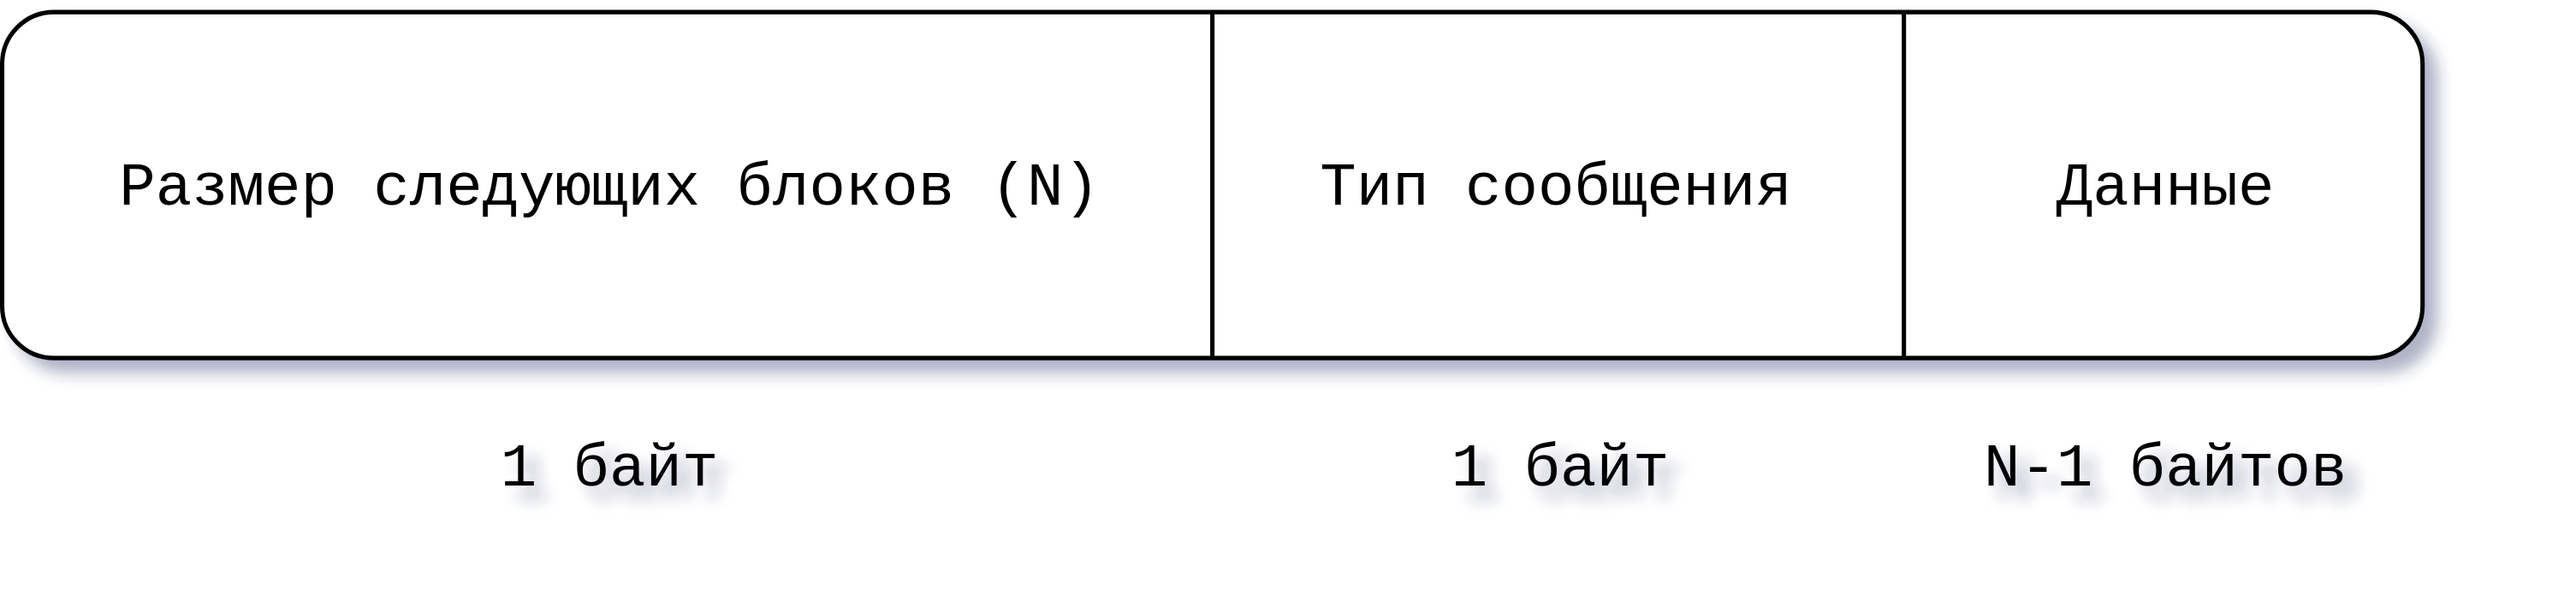
\includegraphics[width=1\textwidth]{CalculatorProtocol}
	\caption{Формат сообщения}
	\label{fig:calc-prot}
\end{figure}

Сообщение разделено на 3 блока:

\begin{enumerate}
	\item Содержит размер следующих блоков в байтах ($N$). Занимает 1 байт
	\item Содержит тип сообщения, который занимает 1 байт
	\item Содержит данные, которые занимают $N-1$ байтов 
\end{enumerate}

В таблице \ref{tab:msg-types} представлены возможные типы сообщений и их бинарное представление.

\begin{table}[H]
\begin{center}
	\caption{Типы сообщений}
	\label{tab:msg-types}
	\def\tabcolsep{10pt}
	\def\arraystretch{1.23}
	\begin{tabular}{|c|c|c|}
		\hline 
		& Тип сообщения & Бинарное представление \\ 
		\hline 
		1 & Математический запрос & $0000\text{ }0000$ \\ 
		\hline 
		2 & Ответ на математический запрос & $0000\text{ }0001$ \\ 
		\hline 
		3 & Управляющий запрос & $0000\text{ }0010$ \\ 
		\hline 
		4 & Ответ на управляющий запрос & $0000\text{ }0011$ \\ 
		\hline 
	\end{tabular} 
\end{center}
\end{table}

Ниже представлен формат данных для каждого типа сообщения:

\begin{enumerate}
	\item \textbf{Математический запрос}.
	
	Формат данных приведен на рис. \ref{fig:math-req}
	
	\begin{figure}[H]
		\centering
		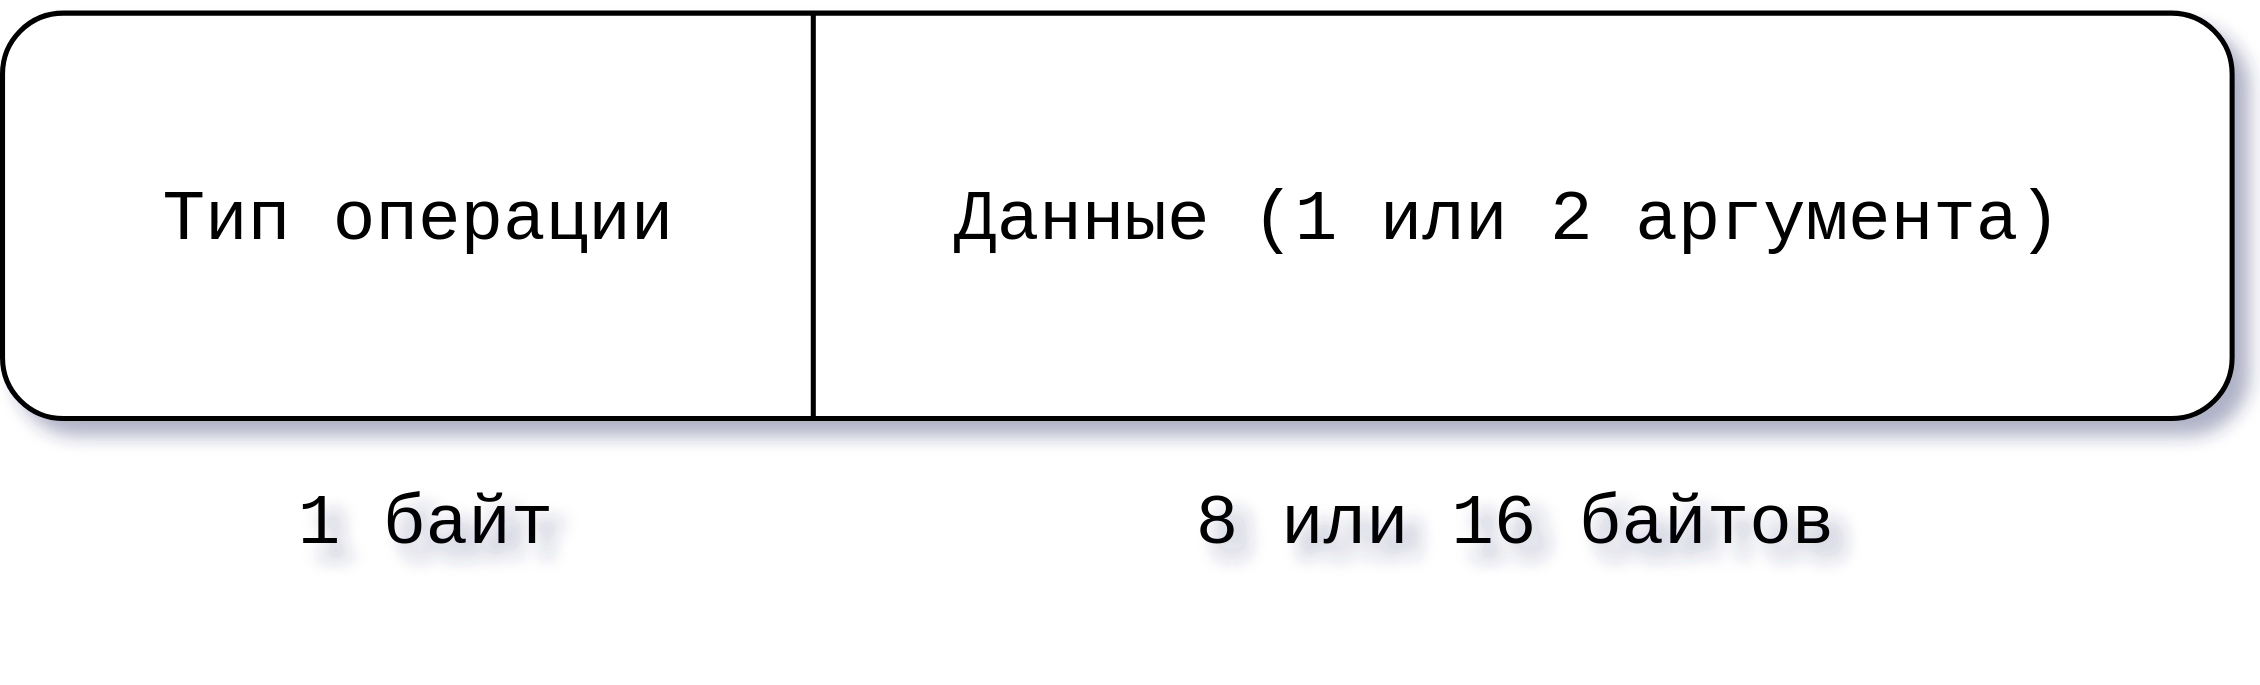
\includegraphics[width=0.8\textwidth]{MathOperation}
		\caption{Формат данных математического запроса}
		\label{fig:math-req}
	\end{figure}
	
	Данные разделены на 2 блока: тип операции, который занимает 1 байт, и данные (аргументы), которые занимают 8 байтов, если для данного типа операции необходим 1 операнд, или 16 байтов, если -- 2 операнда.
	
	В таблице \ref{tab:msg-types} представлены возможные типы операций, их бинарное представление и соответствующее количество аргументов.

	Операнды в бинарном виде кодируются <<старшими байтами вперёд>>.

	\begin{table}[H]
	\begin{center}
		\caption{Типы операций}
		\label{tab:msg-types}
		\def\tabcolsep{4pt}
		\begin{tabular}{|c|c|c|c|}
			\hline 
			& Тип операции & Бинарное представление & Число операндов \\ 
			\hline 
			1 & Сложение & $0000\text{ }0000$ & 2\\ 
			\hline 
			2 & Вычитание & $0000\text{ }0001$ & 2\\ 
			\hline 
			3 & Умножение & $0000\text{ }0010$ & 2\\ 
			\hline 
			4 & Деление & $0000\text{ }0011$ & 2\\ 
			\hline
			5 & Квадратный корень & $0000\text{ }0100$ & 1\\ 
			\hline 
			6 & Факториал & $0000\text{ }0101$  & 1\\ 
			\hline 
		\end{tabular} 
	\end{center}
	\end{table}
	
	\item \textbf{Ответ на математический запрос}.
	%TODO
	
	
\end{enumerate}

\section{Описание архитектур}
%приложений на основе TCP и UDP, их особенностей и ограничений (с графическими схемами

\section{Особенности реализации}
%сетевых и многопоточных приложений: readn, завершение потоков, мьютексы и др
\section{Результаты тестирования}
%приложения (с разным набором входных данных, методика тестирования параллельности обработки запросов клиентов, проверка программы на потерю, дублирование и перемешивание дейтаграмм) .

\section{Выводы}
%Анализ выполненных заданий, сравнение удобства/эффективности/количества проблем при программировании TCP/UDP. Если для реализации прикладного протокола поверх UDP потребовалась модификация прикладного протокола, упомянуть эти измнения. Области применения протоколов TCP и UDP

\end{document}
